\documentclass[11pt]{beamer}
\usetheme[progressbar=frametitle]{metropolis}
%\usetheme{Singapore}
\usepackage[utf8]{inputenc}
\usepackage[spanish]{babel}
\usepackage{fancyvrb}
\definecolor{new_green}{HTML}{347F1F}


\author{Lic. Agustina Pesce \\ Lic. Santiago Soler}
\title[Taller de {\LaTeX}]{Taller Introductorio a {\LaTeX}: \\ Cómo producir documentos de Calidad}
\subtitle{Primer Encuentro: Introducción}
%\setbeamercovered{transparent} 
%\setbeamertemplate{navigation symbols}{} 
%\logo{} 
%\institute{} 
\date{}
%\subject{} 
\begin{document}

\maketitle

\section{Bienvenidos al Taller}

\begin{frame}{Taller Introductorio a {\LaTeX}}
Página del Taller:
%\vspace{1em}
\begin{center}
\textbf{https://santis19.github.io/taller-latex}
\end{center}

\metroset{block=fill}
\begin{block}{}
\begin{center}
!No te olvides de anotarte si todavía no lo hiciste!
\end{center}
\end{block}
\end{frame}

\begin{frame}{Taller Introductorio a {\LaTeX}}
\begin{itemize}[<+- | alert@+>] % Con esto hacemos que aparezcan los items de a uno
  \item ¿Cuáles son los objetivos del Taller?
  \item ¿Cómo los vamos a evaluar?
  \item ¿Y cuántas veces vamos a tener que venir?
\end{itemize}

\pause
\textbf{Cronograma Tentativo}


\begin{enumerate}
  \item Primer Encuentro: Introducción
  \item Segundo Encuentro: Artículo
  \item Tercer Encuentro: Bibliografía
  \item Cuarto Encuentro: Libro
  \item Quinto Encuentro: Clase de Documento de Elsevier
  \item Sexto Encuentro: Herramientas varias y cierre del curso
\end{enumerate}

\end{frame}


\section{¿Qué es {\LaTeX}?}


\begin{frame}{Editores de texto que todos conocemos}
\pause
\textbf{Editores WYSIWYG (What You See Is What You Get)}
\begin{columns}
\column{0.33\textwidth}
\begin{itemize}
  \item \small{Microsoft Word}
\end{itemize}  
\column{0.33\textwidth}
\begin{itemize}
  \item \small{LibreOffice Writer}
\end{itemize}
\column{0.33\textwidth}
\begin{itemize}
  \item \small{Otros}
\end{itemize}
\end{columns}

\begin{figure}[b]
  \centering
  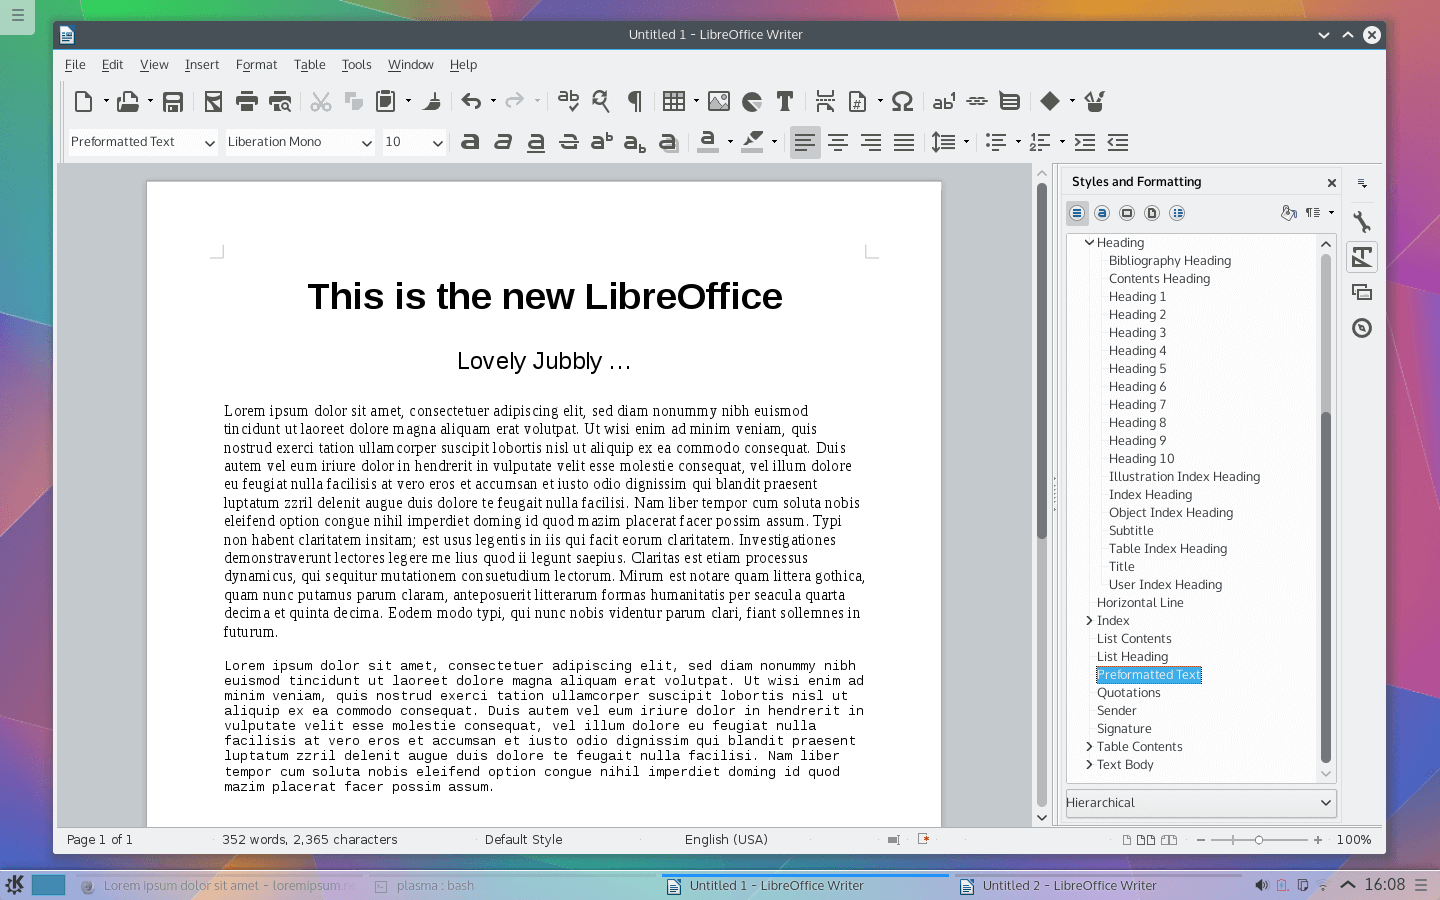
\includegraphics[width=0.9\textwidth]{figs/libreoffice-writer-sample.png}
\end{figure}
\end{frame}

\begin{frame}{{\LaTeX}: un sistema de composición de textos distinto}
\textbf{Editores WYSIWYM (What You See Is What You Mean)}
\begin{figure}
\centering
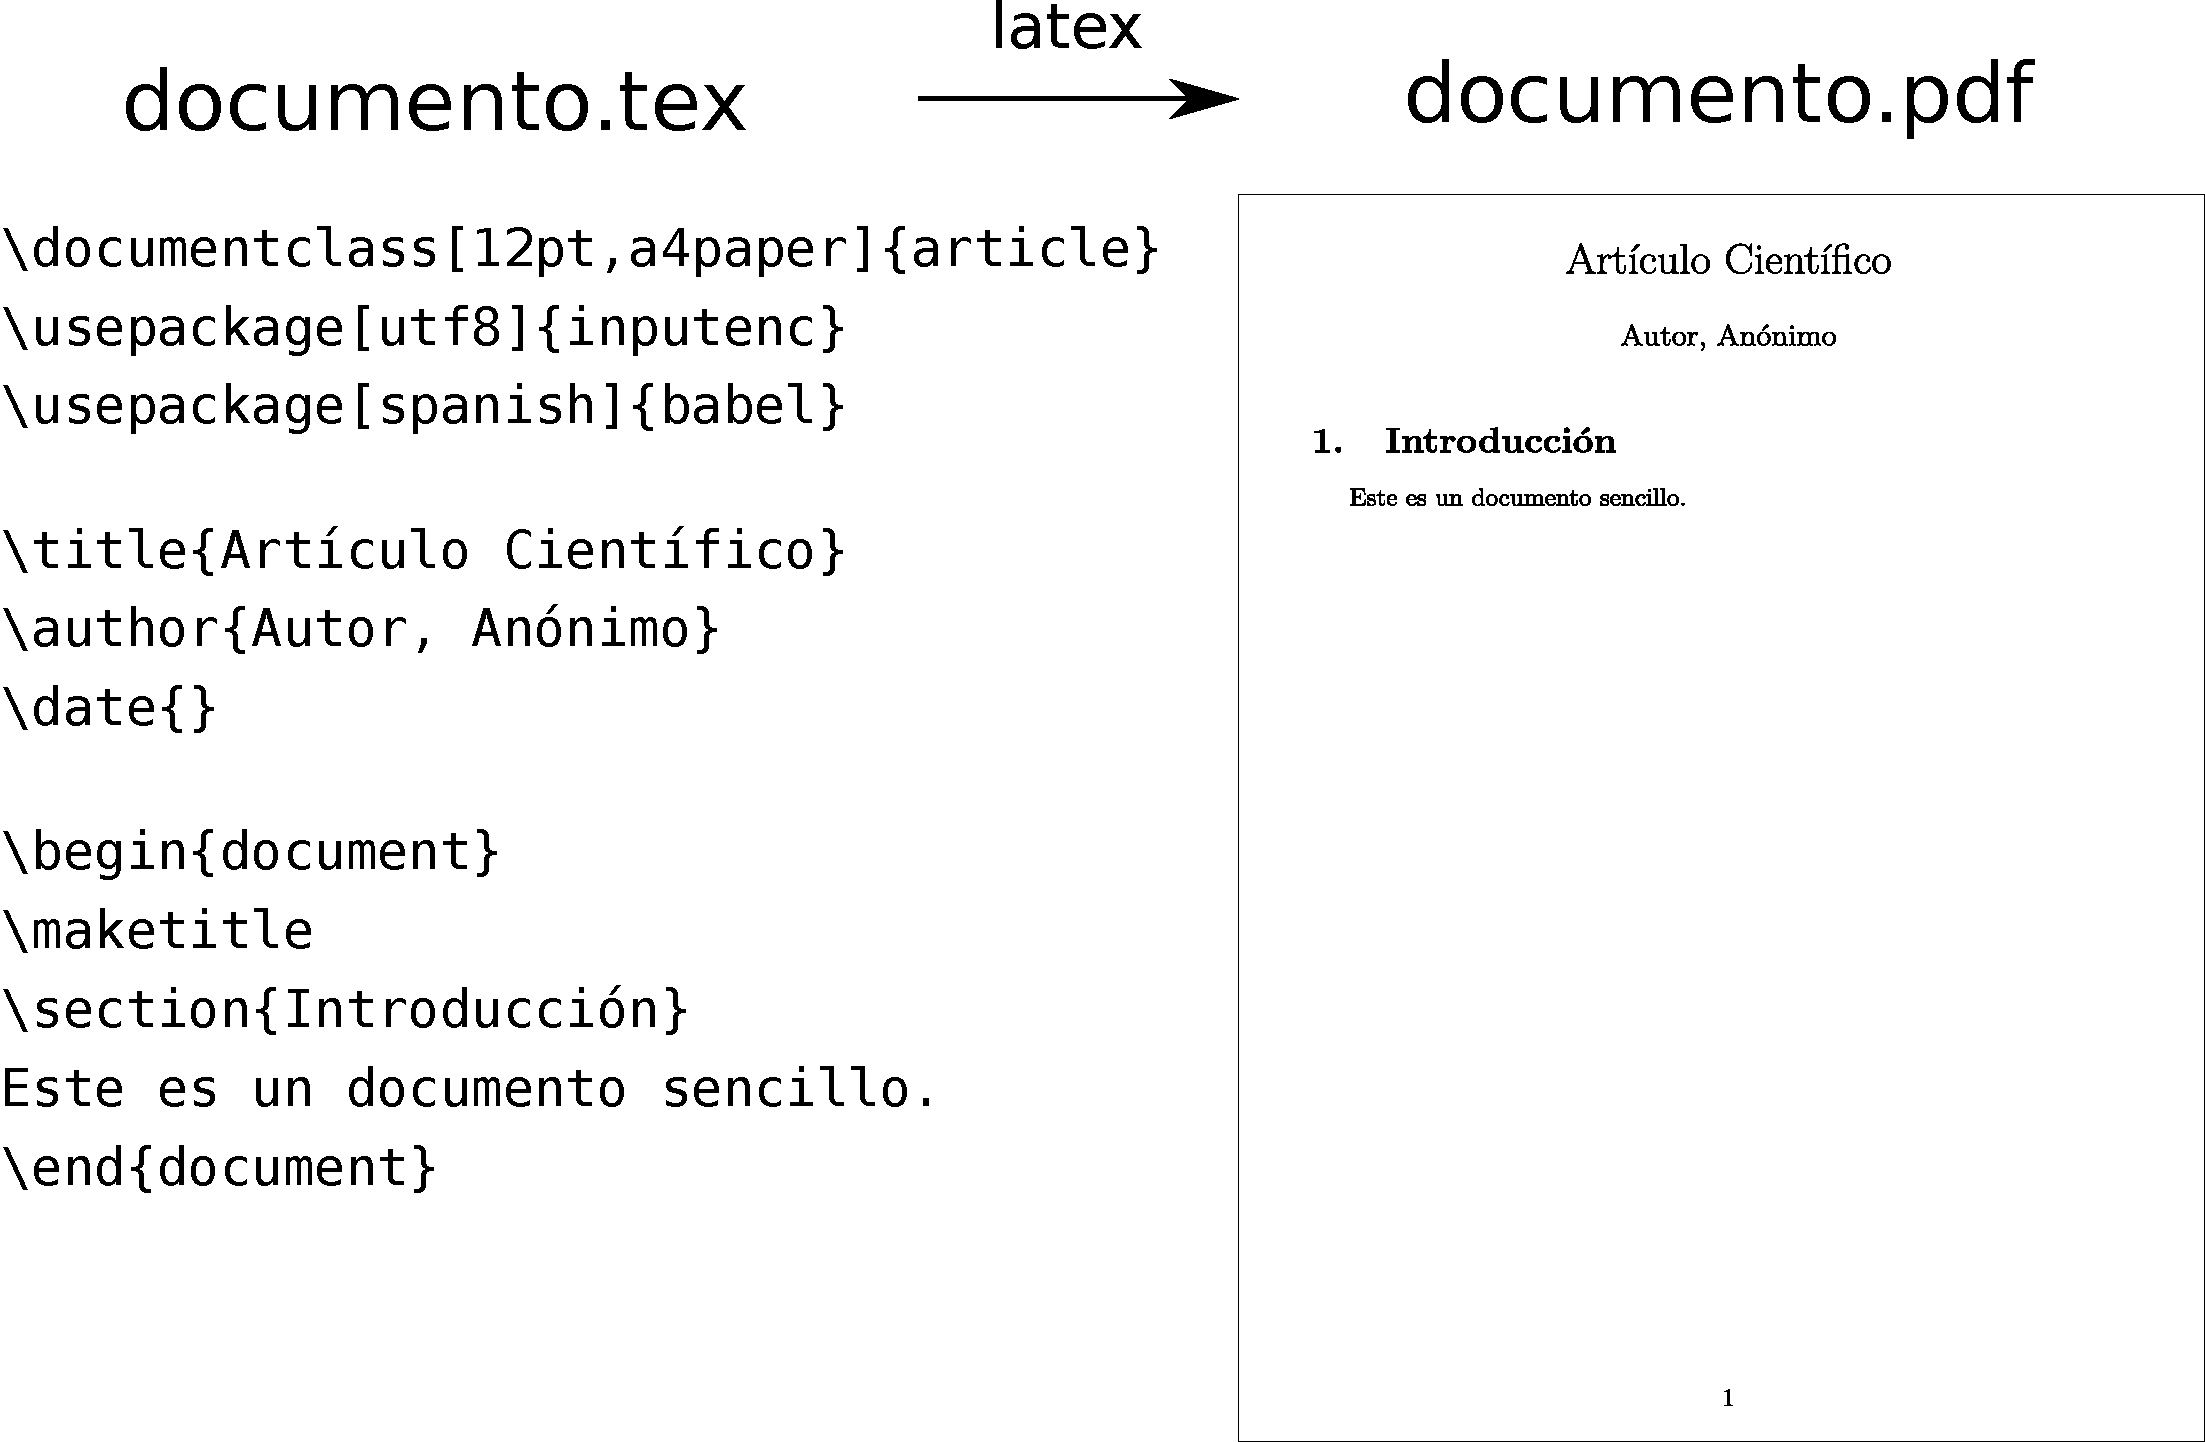
\includegraphics[width=0.9\textwidth]{figs/tex-to-pdf.pdf}
\end{figure}
\end{frame}

\begin{frame}{¿Qué es {\LaTeX}?}

\metroset{block=fill}
\begin{block}{Definición}
{\LaTeX} es un sistema de composición de textos, orientado a la creación de documentos escritos que presenten una alta calidad tipográfica.
\end{block}

\begin{itemize}
\item \TeX{} es un sistema de tipografía escrito por Donald E. Knuth en 1978 diseñado para publicar texto y fórmulas matemáticas con gran calidad tipográfica.
\item {\LaTeX} es un conjunto de macros para {\TeX} escrito por Leslie Lamport en 1984 con el propósito de simplificar el manejo de {\TeX}, pero utilizándolo como motor tipográfico.
\end{itemize}
\end{frame}

\begin{frame}{Ventajas de \LaTeX}
\begin{itemize}[<+- | alert@+>]
  \item Produce documentos de altísima calidad de manera automática siguiendo estándares estéticos.
  \item Nos permite dedicar más tiempo al contenido del documento y menos a su edición.
  \item Permite escribir fórmulas matemáticas de altísima calidad.
  \item Estructuras complejas como referencias cruzadas, notas al pie de página, sangría, títulos, tabla de contenidos, bibliografía, etc. son muy sencillas de introducir.
  \item Nos alienta a producir textos bien estructurados, ya que así son los documentos para los que \LaTeX{} está diseñado.
  \item Nos permite dividir nuestro documento en varios archivos. Muy útil a la hora de escribir textos largos como libros o tesis.
  \item Es Software Libre.
\end{itemize}
\end{frame}

\begin{frame}{Software Libre}
\begin{figure}
\centering
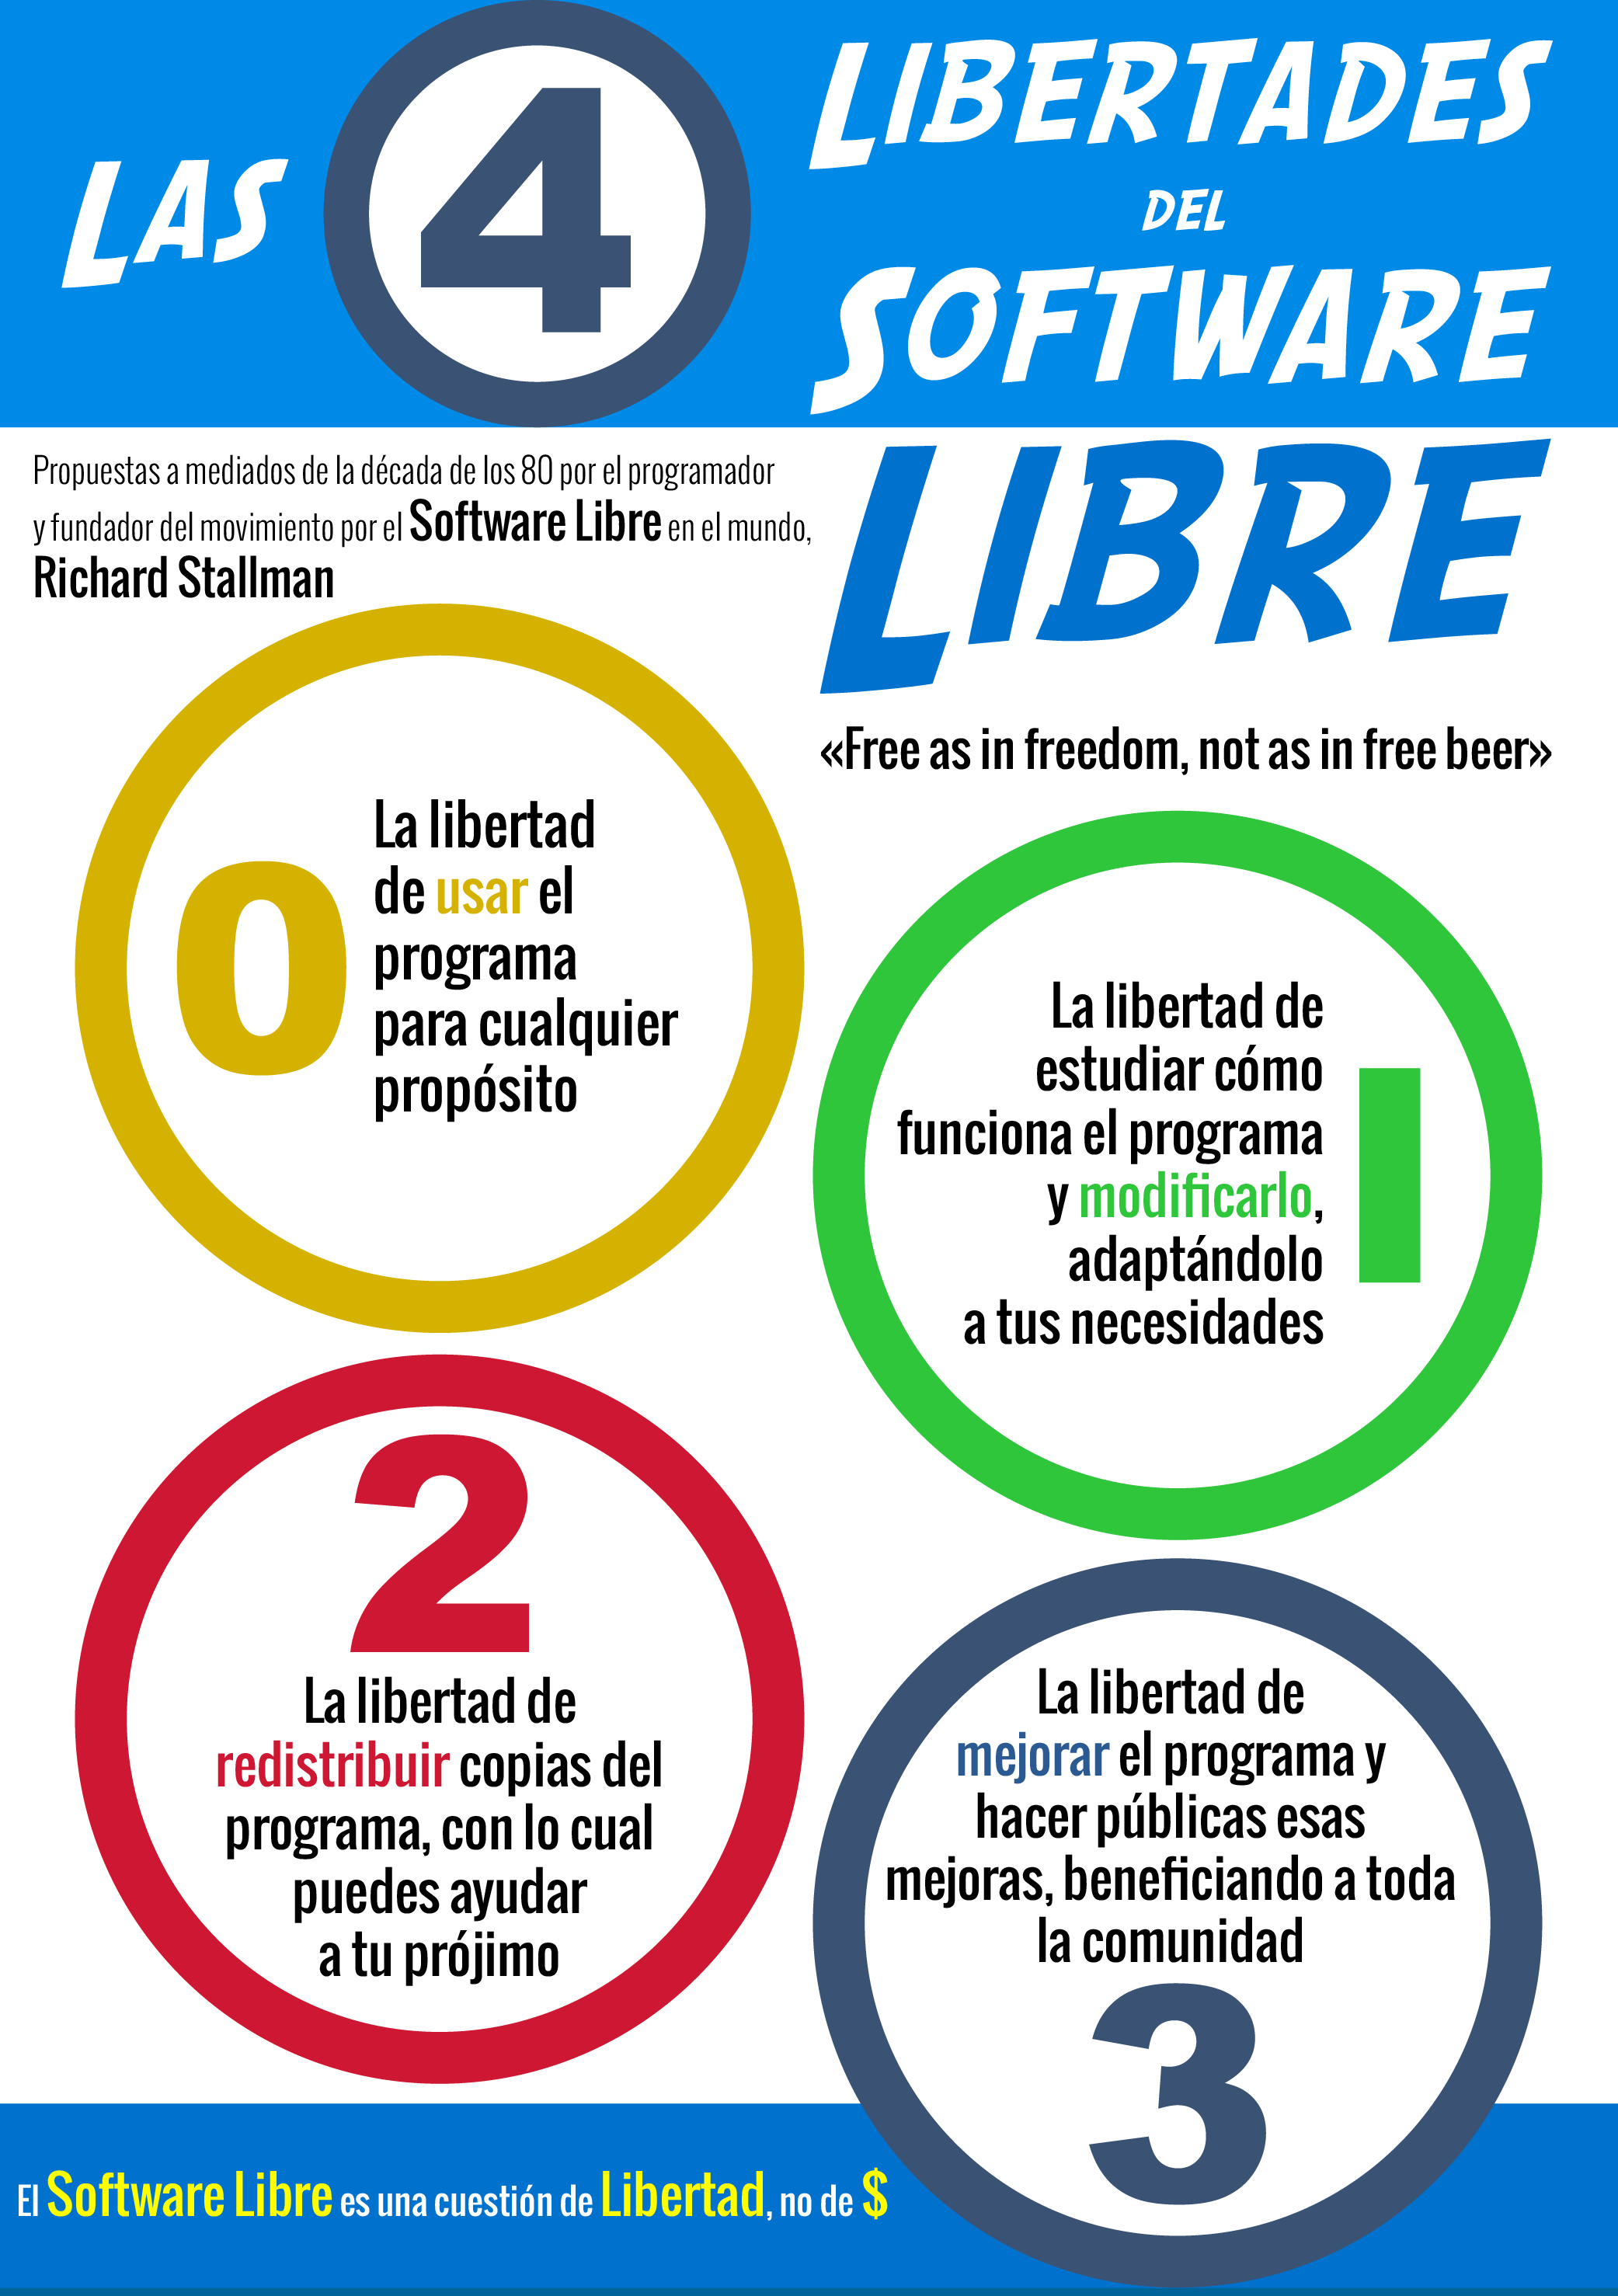
\includegraphics[width=0.52\textwidth]{figs/free-software.png}
\end{figure}
\end{frame}


\begin{frame}{Desventajas de \LaTeX}
\metroset{block=fill}
\begin{block}{La curva de aprendizaje posee una pendiente elevada al principio}
Una vez que la superamos nos permite ser más productivos en comparación con un WYSIWYG.
\end{block}

\pause
\begin{block}{No visualizamos el documento definitivo hasta compilar}
Suele incomodar al principio, pero luego nos ahorra tiempo ya que no nos distraemos con la edición del formato.
\end{block}
\end{frame}

\begin{frame}{Desventajas de \LaTeX}
\metroset{block=fill}
\begin{block}{Solemos tener que lidiar con errores de compilación}
Compilando periódicamente nos facilitará la tarea de identificar esos errores en vez de acumularlos.
\end{block}

\pause
\begin{block}{Producir documentos con un formato no estructurado y arbitrario puede ser engorroso}
{\LaTeX} parte de comandos predefinidos, por ende, generar un documento con un formato nuevo requiere reescribir los estilos o bien ``forzar'' nuestro archivo .tex a que genere un documento similar al que deseamos.
\end{block}
\end{frame}

\begin{frame}{\LaTeX{} vs WYSIWYG}
\begin{figure}
\centering
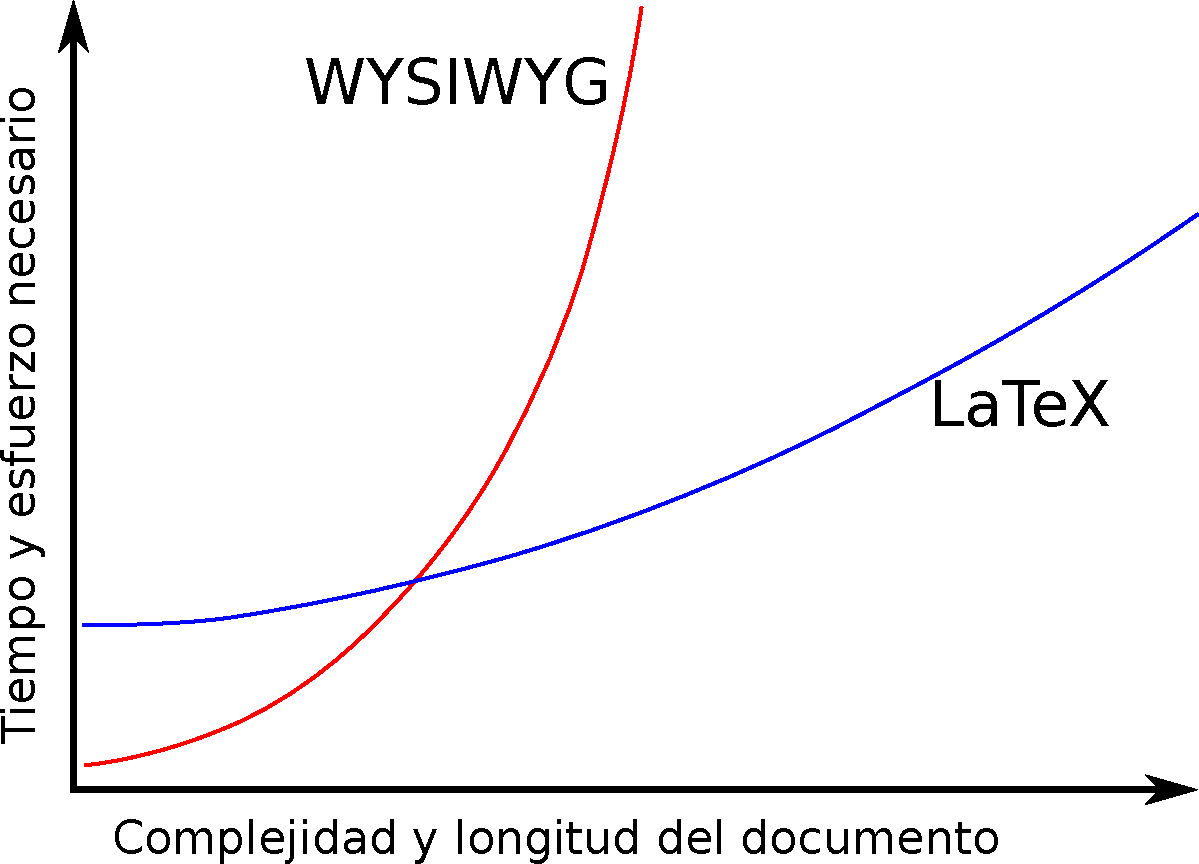
\includegraphics[width=\textwidth]{figs/latex-vs-wysiwyg.pdf}
\end{figure}
\end{frame}


\section{Software Necesario para el Taller}
\begin{frame}[fragile]{Software Necesario para el Taller}
Vamos a necesitar una distribución de \LaTeX{}, un editor y un administrador de bases de datos bibliográficas.

\vspace{1em}

\begin{columns}
\column{0.5\textwidth}
\metroset{block=fill}
\begin{block}{\small GNU/Linux}
\begin{footnotesize}
\begin{description}[fontsize=\small]
  \item[Texlive:] Distribución de \LaTeX{}
  \item[TexMaker:] Editor \LaTeX{}
  \item[JabRef:] Administrador de Base de Datos Bibliográficas
\end{description}
\end{footnotesize}
\end{block}

\column{0.5\textwidth}
\metroset{block=fill}
\begin{block}{\small Windows}
\begin{footnotesize}
\begin{description}[fontsize=\small]
  \item[MikTex:] Distribución de \LaTeX{}
  \item[TexMaker:] Editor \LaTeX{}
  \item[JabRef:] Administrador de Base de Datos Bibliográficas
\end{description}
\end{footnotesize}
\end{block}
\end{columns}

\end{frame}

\section{Hola Mundo en \LaTeX}
\begin{frame}[fragile]{Hola Mundo en \LaTeX}
\begin{enumerate}
\item Creamos una carpeta donde vamos a colocar todos los archivos necesarios para la creación de nuestro articulo
\item El archivo \LaTeX{} tendrá la extensión .tex
% Mostramos en vivo el TexMaker. TexMaker > Asistente > Crear Doc. Nuevo > Article
\item Nuestro primer documento: \\
{\color{new_green}
\begin{verbatim}
\documentclass[12pt,a4paper]{article}
\usepackage[utf8]{inputenc}
\usepackage[spanish]{babel}

\begin{document}
Hola Mundo
\end{document}
\end{verbatim}
}
\item Compilamos: \LaTeX{} genera un .pdf en la carpeta del proyecto
% Explicar archivos auxiliares, qué es lo importante -> .tex
\end{enumerate}
\end{frame}

\section{Estructura y Sintaxis de Documentos \LaTeX{}}

\begin{frame}[fragile]{Estructura básica de un documento \LaTeX}

\textbf{Estructura básica}

Un documento básico de \LaTeX{} se compone de dos partes:
\begin{itemize}
\item Preámbulo del documento
{\color{new_green}
\begin{verbatim}
\documentclass[12pt,a4paper]{article}
\usepackage[utf8]{inputenc}
\usepackage[spanish]{babel}
\end{verbatim}
}
\item Cuerpo del documento
{\color{new_green}
\begin{verbatim}
\begin{document}
Este es el cuerpo de mi documento.
\end{document}
\end{verbatim}
}
\end{itemize}


\end{frame}

\begin{frame}[fragile]{Espacios y Párrafos}

\metroset{block=fill}
\begin{block}{Espacios en blanco}
Los espacios en blanco y tabulaciones son tratados como simples espacios por \LaTeX{}. Múltiples espacios son considerados como un único espacio. Los espacios al inicio del párrafo son ignorados.
\end{block}

\metroset{block=fill}
\begin{block}{Párrafos}
Los párrafos deben ser separados por una línea en blanco.
\end{block}

\vspace{1em}

\begin{columns}
\column{0.5\textwidth}
{\color{new_green}
\begin{Verbatim}[fontsize=\footnotesize]
   No importa si ponemos muchos 
espacios      entre palabras.
   
La línea en blanco indica que 
terminó el párrafo anterior y 
comienza uno nuevo.
\end{Verbatim}
}
\column{0.5\textwidth}
   No importa si ponemos muchos 
espacios      entre palabras.
   
La línea en blanco indica que 
terminó el párrafo anterior y 
comienza uno nuevo.
\end{columns}

\end{frame}


\begin{frame}[fragile]{Caracteres Especiales}
\metroset{block=fill}
\begin{block}{Caracteres Especiales}
Los siguientes símbolos son caracteres reservados que poseen un significado especial para \LaTeX. Si los introducimos directamente no va a imprimirlos en el pdf, sino que hará que \LaTeX se comporte de forma que no deseamos.
\end{block}

\begin{center}
\# \$ \% \^{} \& \_ \{ \} \~{} \textbackslash
\end{center}

Para introducirlos debemos hacerlo de la siguiente manera:
\begin{center}
{\color{new_green}
\begin{Verbatim}
\# \$ \% \^{} \& \_ \{ \} \~{} \textbackslash
\end{Verbatim}
}
\end{center}

\end{frame}

\begin{frame}[fragile]{Caracteres Especiales}
\metroset{block=fill}
\begin{block}{Comillas}
Las comillas deben escribirse de la siguiente forma:
\end{block}

\begin{columns}
\column{0.5\textwidth}
{\color{new_green}
\begin{Verbatim}
``comillas''
\end{Verbatim}
}
\hfill
\column{0.5\textwidth}
``comillas''
\end{columns}


\begin{block}{Comentarios en texto}
Utilizando el símbolo \% podemos agregar comentarios en el texto que no serán impresos en el .pdf
\end{block}

\begin{columns}
\column{0.5\textwidth}
{\color{new_green}
\begin{Verbatim}
Este texto tiene un
comentario % comentario
\end{Verbatim}
}
\hfill
\column{0.5\textwidth}
Este texto tiene un
comentario % comentario
\end{columns}

\end{frame}

\section{Comandos y Paquetes}

\begin{frame}[fragile]{Comandos}
\metroset{block=fill}
\begin{block}{Comandos \LaTeX}
Los comandos de \LaTeX{} comienzan con una barra invertida: \textbackslash
\end{block}

\textbf{Ejemplos:}
\begin{columns}
\column{0.5\textwidth}
{\color{new_green}
\begin{verbatim}
\textbf{Texto en negrita}
\textit{Texto en italic}
{\small Texto small}
{\huge Texto huge}
\end{verbatim}
}
\hfill
\column{0.5\textwidth}
\textbf{Texto en negrita} \\
\textit{Texto en italic} \\
{\small Texto small} \\
{\huge Texto huge}
\end{columns}

\vspace{-1em}
\metroset{block=fill}
\begin{block}{Otros comandos \LaTeX}
Otros comandos \LaTeX{} más complejos tienen la siguiente sintaxis:
\vspace{-1em}
\begin{verbatim}
\comando[opciones]{parámetro}
\end{verbatim}
\end{block}
\end{frame}


\begin{frame}[fragile]{Comandos}

Otro ejemplo de comandos en \LaTeX{} es \textbf{pagestyle}. Este comando nos permite modificar la aparición de la numeración de página en encabezado o pie de página.
El siguiente comando elimina la numeración de todas las páginas:
{\color{new_green}
\begin{verbatim}
\pagestyle{empty}
\end{verbatim}
}


Si en cambio, deseamos eliminar la numeración de una página en particular podemos utilizar:
{\color{new_green}
\begin{verbatim}
\thispagestyle{empty}
\end{verbatim}
}

\end{frame}


\begin{frame}[fragile]{Comandos}

Otros parámetros para el comando pagestyle pueden ser:

{\small
\begin{description}
\item [plain] Los números se sitúan en el pie de página. Es el estilo predeterminado.
\item [headings] La numeración se sitúa en el encabezado, junto con el nombre de la sección.
\item [empty] Produce páginas sin numeración.
\end{description}
}

\end{frame}


\begin{frame}[fragile]{Paquetes}

Muchas veces nos encontraremos que \LaTeX{} no puede resolver nuestros problemas por sí solo. En esos casos es necesario incluir ``mejoras'' a nuestro documento, y eso lo hacemos a través del uso de \textbf{paquetes}.

En caso de querer usar un paquete en particular, tenemos que agregar una línea como la siguiente en el preámbulo:

{\color{new_green}
\begin{verbatim}
\usepackage[options]{package-name}
\end{verbatim}
}

\end{frame}

\begin{frame}[fragile]{Paquetes}

Por ejemplo, si queremos modificar la geometría de nuestra hoja cambiando el ancho de los márgenes, necesitamos utilizar el paquete \textbf{geometry} junto con las medidas de los márgenes como opciones.

{\color{new_green} \small
\begin{verbatim}
\usepackage[hmargin=2.5cm,vmargin=2.5cm]{geometry}
\end{verbatim}
}

También podemos modificar los márgenes individualmente:

{\color{new_green} \small
\begin{verbatim}
\usepackage[left=3cm,right=2cm,top=2.5cm,bottom=2.5cm]{geometry}
\end{verbatim}
}

\end{frame}


\section{Fórmulas Matemáticas}

\begin{frame}[fragile]{Fórmulas Matemáticas}
\metroset{block=fill}
\begin{block}{Fórmulas matemáticas}
\LaTeX{} nos permite escribir ecuaciones y símbolos matemáticos de forma muy sencilla. Para hacerlo usaremos el símbolo \$ para indicar el inicio y el final de una ecuación en línea. Y utilizamos dos \$\$ para situar la ecuación en una línea propia.
\end{block}

\textbf{Ejemplo:}

Esta es una ecuación en línea: $E = mc^2$
\vspace{-1em}
{\color{new_green}
\begin{verbatim}
Esta es una ecuación en línea: $E = mc^2$
\end{verbatim}
}

Esta es una ecuación en su propia línea: 
$$E = mc^2$$

\vspace{-1em}
{\color{new_green}
\begin{verbatim}
Esta es una ecuación en su propia línea:
$$E = mc^2$$
\end{verbatim}
}
\end{frame}

\begin{frame}[fragile]{Entorno Equation}
\metroset{block=fill}
\begin{block}{Entornos}
\LaTeX{} posee estructuras llamadas entornos que se abren con \textbackslash begin\{entorno\} y se cierran con \textbackslash end\{entorno\}
\end{block}

\metroset{block=fill}
\begin{block}{Entorno Equation}
Uno de los entornos que utilizaremos es el ``equation''. Nos permite numerar la ecuación y luego hacer referencia a ella.
\end{block}

\vspace{-1em}

\textbf{Ejemplo:}

\vspace{-1em}

\begin{verbatim}
\begin{equation}
\sum_{k=0}^{n-1} ak^r = a \frac{1-r^n}{1-r}
\end{equation}
\end{verbatim}

\vspace{-2em}

\begin{equation}
\sum_{k=0}^{n-1} ak^r = a \frac{1-r^n}{1-r}
\end{equation}
\end{frame}


\end{document}
